\RequirePackage[dvipsnames]{xcolor}
\documentclass[10pt]{NSP1}
\usepackage{url,floatflt}
\usepackage{helvet,times}
\usepackage{psfig,graphics}
\usepackage{mathptmx,amsmath,amssymb,bm}
\usepackage{float}
\usepackage[bf,hypcap]{caption}
\usepackage{booktabs}


\tolerance=1
\emergencystretch=\maxdimen
\hyphenpenalty=10000
\hbadness=10000

\topmargin=0.00cm

\def\sm{\smallskip}
\def\no{\noindent}

\def\firstpage{1}
\setcounter{page}{\firstpage}
\def\thevol{20}
\def\thenumber{5}
\def\theyear{2026}

\begin{document}

    \titlefigurecaption{{\large \bf \rm Applied Mathematics \& Information Sciences }\\ {\it\small An International Journal}}

    \title{Bessel Moment Polynomials}

\author{Héctor M. Moya-Cessa}
\institute{Instituto Nacional de Astrofísica Óptica y Electrónica, Calle Luis Enrique Erro No. 1, Santa María Tonantzintla, Pue., 72840, Mexico.}

    \titlerunning{Bessel Moment Polynomials}
    \authorrunning{Héctor M Moya-Cessa}

    %corresponding author email
    \mail{hmmc@inaoep.mx}

    \received{22 Dec. 2020}
    \revised{2 Jan. 2020}
    \accepted{24 Jan. 2020}
    \published{1 Mar. 2021}

\abstracttext{We study the family of even moments of squared Bessel functions of the first kind,
\[
\mathcal{P}_n(x)=\sum_{k=0}^{\infty}k^{2n}\,J_k^2(2x),\qquad n\ge 1.
\]
By means of the classical generating--function identity 
$\sum_{k=-\infty}^{\infty}J_k^2(a)e^{iky}=J_0(2a\sin y/2)$, 
we prove that each $\mathcal{P}_n$ is an even polynomial of degree $2n$ in $x$, 
or equivalently a polynomial $p_n(u)$ of degree $n$ in the variable $u=x^2$.  
We derive an explicit formula for the coefficients $a_{n,m}$ and establish a three--term 
recurrence relation.  The first few polynomials are
\[
\begin{aligned}
p_1(u)&=u,\\
p_2(u)&=3u^2+u,\\
p_3(u)&=10u^3+15u^2+u,\\
p_4(u)&=35u^4+140u^3+63u^2+u,\\
p_5(u)&=126u^5+1050u^4+1470u^3+255u^2+u.
\end{aligned}
\]
All formulas are verified numerically with tight truncation--error bounds.}

\keywords{Schr\"{o}dinger equation; polynomials; generalized Bessel functions; special functions; nonlinear coherent states.}

\maketitle

\section{Introduction}
\label{sec:intro}

Bessel functions of the first kind, $J_k(z)$, are among the most ubiquitous special functions 
in mathematical physics.  They emerge naturally in problems possessing circular or cylindrical 
symmetry, in the theory of diffraction, in signal processing, and in the quantum mechanics of 
periodic systems~\cite{Watson,Gradshteyn,NIST,Axioms}.  In particular, the propagation of classical 
electromagnetic fields in weakly coupled optical waveguide arrays is governed by discrete 
Schr\"{o}dinger--type equations whose eigenfunctions are precisely Bessel functions of 
integer order~\cite{Jones,Makris}.  This observation has fueled a productive analogy between 
classical light propagation and quantum electrodynamics: under appropriate conditions, the 
interaction between quantized light and matter can be modelled classically by suitably 
engineered optical lattices~\cite{LonghiI,LonghiII,CrispI,CrispII,ScriptaT}.

A prominent example is the Jaynes--Cummings model \cite{Several,Book} and its generalisations 
(the Rabi model, the Dicke model, anisotropic and driven variants, etc.), all of which can be 
simulated experimentally by arrays of evanescently coupled waveguides~\cite{Jaynes,Shore,Larson,Chen,BraakI,Anisotropic,Bocanegra,Vidiella,Dicke,BraakII}. Atom-field interactions when only counter rotating terms are considered, {\it  i.e.}, the anti-Jaynes-Cummings model \cite{Lara,Mayero} also may be models. Furthermore, time--dependent couplings, which correspond to bent or curved waveguide arrays, further 
broaden the scope of this analogy and allow one to mimic non--autonomous quantum 
evolutions~\cite{Messina,Tsuitsui}.

In the simplest infinite--array geometry with constant nearest--neighbour coupling, the 
amplitudes of the propagating modes are given exactly by Bessel functions~\cite{Jones,Makris}.  
When the array is semi--infinite the analysis becomes substantially more involved, often 
requiring phase--operator techniques~\cite{London,Susskind}.  A natural extension, in which 
light can hop to several neighbours, leads to generalised Bessel functions that have been 
studied extensively by Dattoli and co--workers~\cite{Dattolia,Dattolib,Dattolic} and more 
recently in the context of multi--site waveguide couplers~\cite{Tapia}.

On the quantum--optical side, nonlinear coherent states whose expansion coefficients are 
Bessel functions have attracted recent attention~\cite{Manko,RevMexFis,Gazeau}.  In order to 
characterise the statistical properties of such states, for instance, to compute the Mandel 
$Q$-parameter \cite{Mandel} one needs closed-form expressions for moments of the number operator, 
which reduce to evaluating sums of the type
\begin{equation}\label{eq:firsteq}
\sum_{k=0}^{\infty}k^{n}\,J_k^2(2x).
\end{equation}
For $n=0$ and $n=1$ the sums are elementary consequences of Bessel's closure identity and 
a classical recurrence.  The cases $n=2$ and $n=3$ can also be computed explicitly, but 
already at $n=3$ the result is a cumbersome combination of Bessel functions of different 
orders, and no clear pattern is discernible for higher odd moments.  

The purpose of the present paper is to show that a \emph{discrete family of even moments}, 
namely
\begin{equation}\label{eq:main}
\mathcal{P}_n(x)=\sum_{k=0}^{\infty}k^{2n}\,J_k^2(2x),\qquad n=1,2,3,\dots,
\end{equation}
possesses a remarkably simple structure: each $\mathcal{P}_n(x)$ is an even polynomial of 
degree $2n$ in $x$.  Setting $u=x^2$ we write $p_n(u)=\mathcal{P}_n(x)$ and refer to the 
family $\{p_n(u)\}_{n\ge 1}$ as \emph{Bessel moment polynomials}.  Our main contributions are:
\begin{itemize}
\item a closed formula for the coefficients $a_{n,m}$ of $p_n(u)$;
\item a three--term recurrence relation linking $p_{n+1}$ to $p_n$; and
\item a generating function for Bessel moment polynomials.

\end{itemize}

The leading coefficients $1,3,10,35,126,\dots$ are one half of the central binomial 
coefficients $\tfrac12\binom{2n}{n}$; to the best of our knowledge have not appeared previously in  the literature on Bessel moments~\cite{Fenyes,Kapteyn,Lommel,OEIS}.


\section{First Moments and Motivation}
\label{sec:first}

Nonlinear coherent states generated by the action of exponential Susskind--Glogower--London 
operators on the vacuum take the form~\cite{RevMexFis,Gazeau}
\begin{equation}\label{Coherent}
|x\rangle_{\mathrm{SGL}}=\frac{1}{x}\sum_{n=0}^{\infty}(n+1)J_{n+1}(2x)\,|n\rangle,
\end{equation}
where $|n\rangle$ denotes the Fock (number) state with $n$ photons.  The normalisation and 
moment sums of this state involve precisely the series~\eqref{eq:firsteq}.  For $n=0$ the 
closure identity for squared Bessel functions,
\begin{equation}
J_0^2(2x)+2\sum_{k=1}^{\infty}J_k^2(2x)=1,
\end{equation}
gives immediately
\begin{equation}
\sum_{k=0}^{\infty}J_k^2(2x)=\frac{1-J_0^2(2x)}{2}.
\end{equation}
The first moment ($n=1$) is a classical identity:
\begin{equation}
\sum_{k=0}^{\infty}k\,J_k^2(2x)=2x^2\bigl[J_0^2(2x)+J_1^2(2x)\bigr]-xJ_0(2x)J_1(2x).
\end{equation}
For $n=2$ the sum can be extracted from the normalisation of~\eqref{Coherent}:
\begin{equation}\label{eq:firsttwo}
\sum_{k=0}^{\infty}k^2\,J_k^2(2x)=x^2.
\end{equation}
The case $n=3$ is already considerably more involved~\cite{RevMexFis}:
\begin{align}
\sum_{k=0}^{\infty}k^{3}\,J_k^2(2x)
&= x^2\Bigl[(6x^2+1)J_0^2(2x)+(6x^2-1)J_1^2(2x)\Bigr] \nonumber\\
&\quad - 2x^3 J_0(2x)J_1(2x) \nonumber\\
&\quad + \frac{2x^4}{3}\Bigl[J_0(2x)J_2(2x)+J_1(2x)J_3(2x)\Bigr].
\end{align}
Figure~\ref{fig_0} displays the logarithm of both sides of this identity, showing perfect 
agreement.  The important observation is that odd moments do \emph{not} appear to close 
polynomially; instead they remain transcendental combinations of Bessel functions.  It is the 
restriction to \emph{even} moments that reveals the hidden polynomial structure.

\begin{figure}[H]
\centering
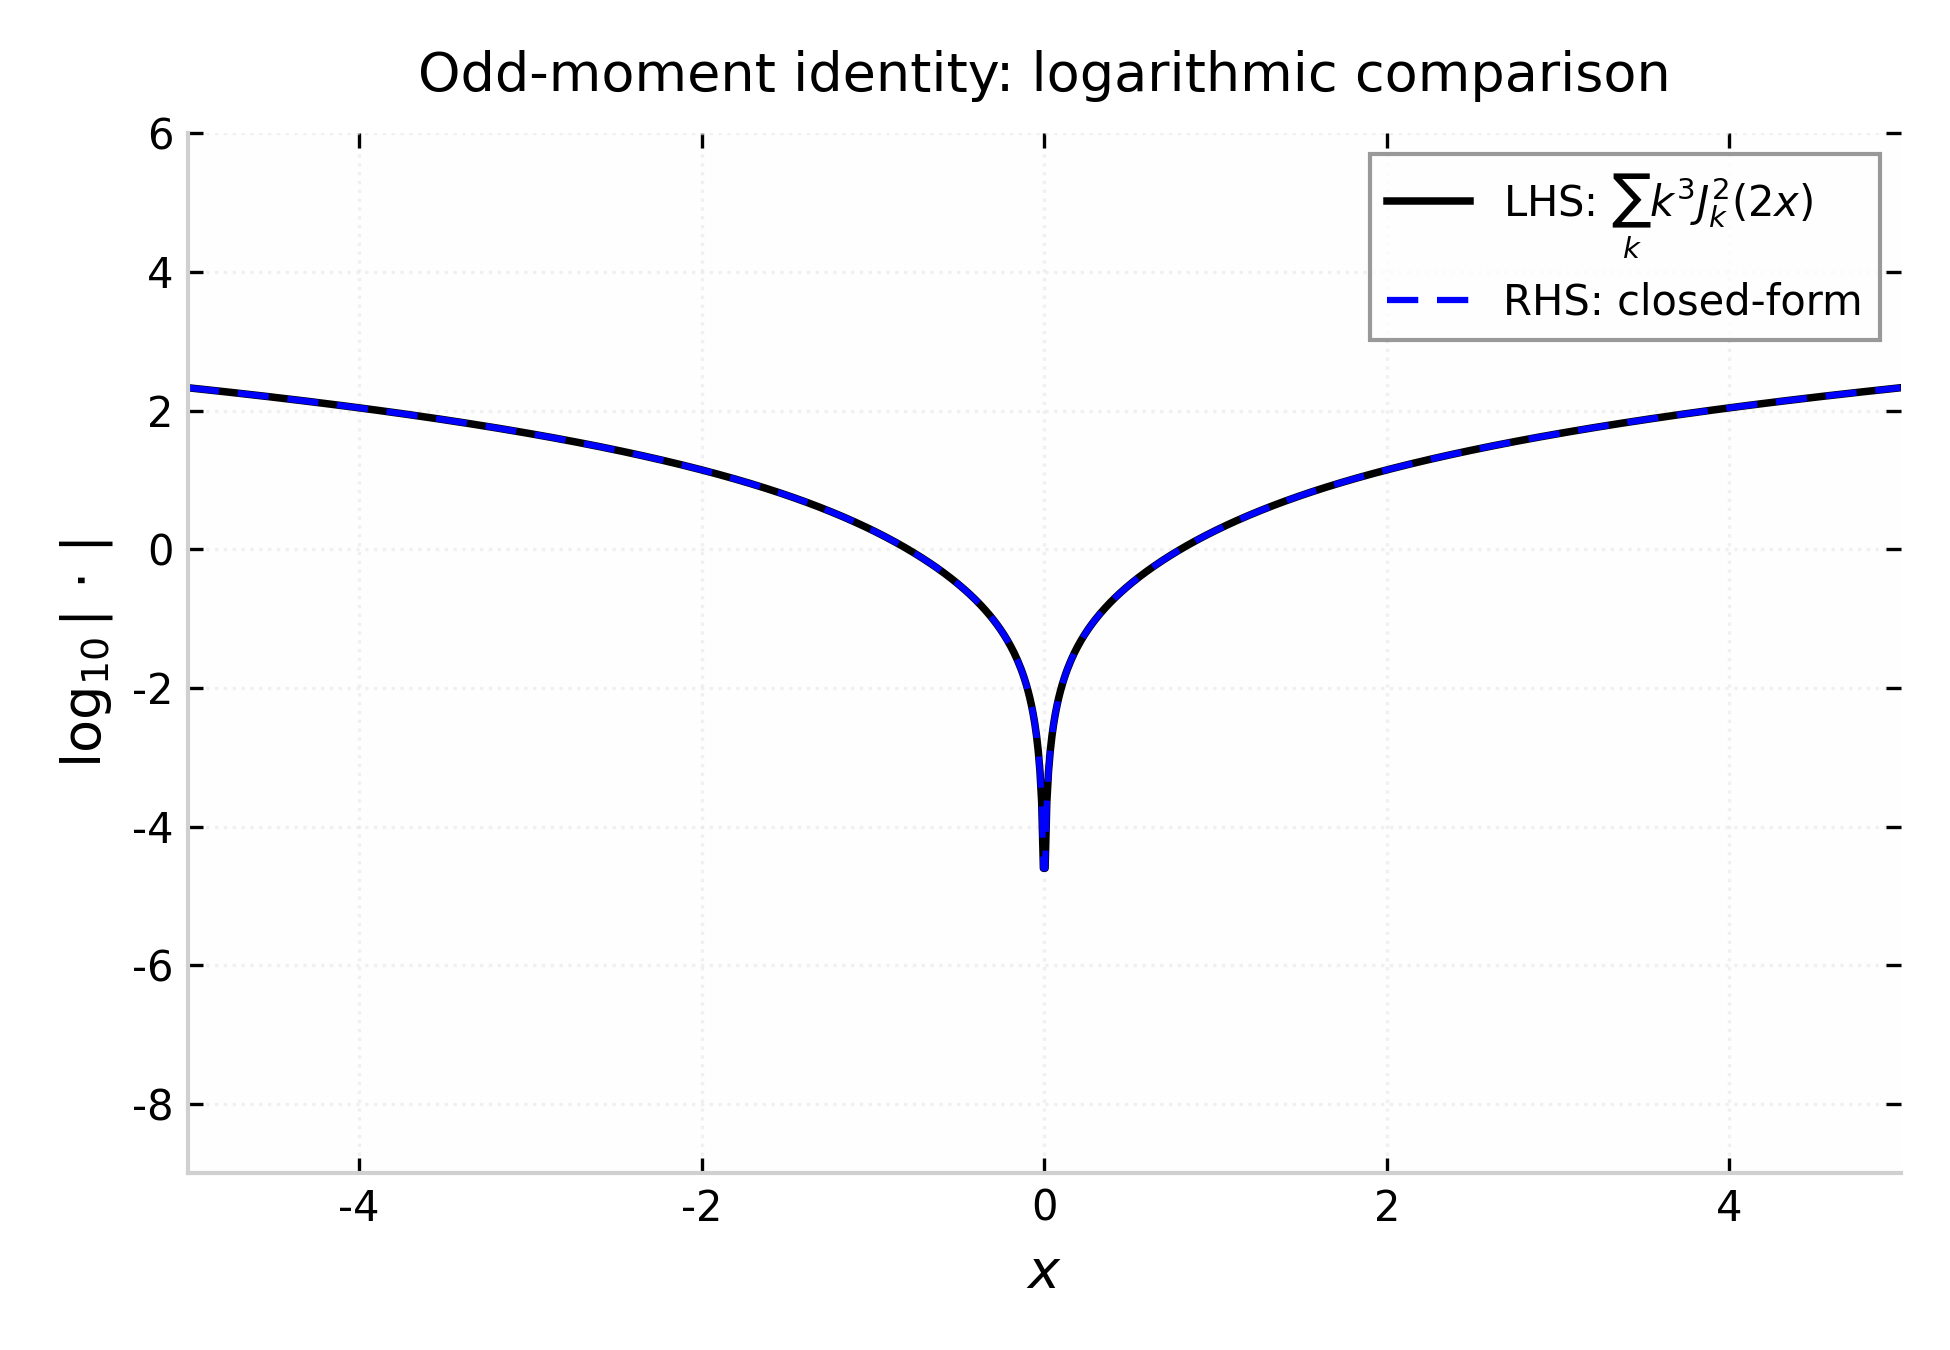
\includegraphics[width=\linewidth]{figure1.png}
\caption{Logarithmic plot of the left--hand side (solid line) and right--hand side (dashed line) 
of the odd--moment identity for $n=3$, showing perfect agreement.}
\label{fig_0}
\end{figure}
\begin{align}
\sum_{k=0}^{\infty} k^{5} J_k^2(2x)
&= x^{2}\left(\frac{50x^{4}}{3}+\frac{52x^{2}}{3}+1\right)J_{0}^{2}(2x) \nonumber\\
&\quad + x^2\left(\frac{50x^{4}}{3}+20x^{2}-\frac{29}{3}\right)J_{1}^{2}(2x) \nonumber\\
&\quad - x^2\left(\frac{28x^{3}}{3}-\frac{4x}{3}\right)J_{0}(2x)J_{1}(2x) \nonumber\\
&\quad + \frac{2x^{6}}{5}\big[J_{0}(2x)J_{4}(2x)+J_{1}(2x)J_{5}(2x)\big].
\end{align}
Henceforth, we concentrate on the even--moment family~\eqref{eq:main}.  It is convenient to 
work in the quadratic variable
\begin{equation}\label{eq:udef}
u=x^2,
\end{equation}
and to define the associated polynomials
\begin{equation}\label{eq:pndef}
p_n(u)=\mathcal{P}_n(x)=\sum_{m=1}^{n}a_{n,m}\,u^{m},\qquad n\ge 1.
\end{equation}
The first few are
\[
\begin{aligned}
p_1(u)&=u,\\
p_2(u)&=3u^2+u,\\
p_3(u)&=10u^3+15u^2+u,\\
p_4(u)&=35u^4+140u^3+63u^2+u,\\
p_5(u)&=126u^5+1050u^4+1470u^3+255u^2+u.
\end{aligned}
\]

\subsection{Relation to Existing Literature}

Moments of the form $\int_0^\infty \nu^n J_\nu(t)\,d\nu$ were investigated by 
F\'{e}nyes~\cite{Fenyes}, who showed that they decompose into a polynomial part plus 
oscillatory corrections.  Kapteyn series~\cite{Kapteyn,Watson}, i.e. sums of the type 
$\sum a_n J_{\nu+n}((\nu+n)z)$, appear in orbital mechanics and radiation problems.  The 
Lommel polynomials $R_{m,\nu}(z)$ satisfy a three--term recurrence and are orthogonal with 
respect to a discrete measure~\cite{Lommel,NIST}.  The Bessel polynomials 
$y_n(x)=\sum_{k=0}^n\frac{(n+k)!}{(n-k)!\,k!}\bigl(\frac{x}{2}\bigr)^k$ and the standard 
orthogonal families (Legendre, Hermite, Laguerre) are likewise distinct from the present 
family.  We therefore believe that the explicit results developed below are new.


\section{Generating Function and Polynomial Structure}
\label{sec:gen}

The starting point of our analysis is the well--known identity~\cite{Watson,Gradshteyn}
\begin{equation}\label{eq:gen}
\sum_{k=-\infty}^{\infty}J_k^2(a)\,e^{iky}=J_0\!\bigl(2a\sin\tfrac{y}{2}\bigr),\qquad y\in\mathbb R.
\end{equation}
For $a=2x$ this becomes
\begin{equation}\label{eq:gen2}
\sum_{k=-\infty}^{\infty}J_k^2(2x)\,e^{iky}=J_0\!\bigl(4x\sin\tfrac{y}{2}\bigr).
\end{equation}
Because $J_{-k}(z)=(-1)^kJ_k(z)$, we have $J_{-k}^2(2x)=J_k^2(2x)$; hence the terms with 
$k$ and $-k$ are equal and the sum is an even function of $y$.

\begin{proposition}\label{prop:poly} \,
For every integer $n\ge 1$ the sum~\eqref{eq:main} is a polynomial in $u=x^2$ of degree 
exactly $n$.  In particular, the representation~\eqref{eq:pndef} holds for suitable rational 
coefficients $a_{n,m}$.
\end{proposition}

\begin{proof}
Differentiate~\eqref{eq:gen2} $2n$ times with respect to $y$ and set $y=0$.  Since 
$J_0(4x\sin y/2)$ is an even, analytic function of $y$, all odd derivatives vanish at the 
origin.  Using $\frac{d^{2n}}{dy^{2n}}e^{iky}\big|_{y=0}=(-1)^n k^{2n}$, we obtain
\begin{equation}\label{eq:moment}
\sum_{k=-\infty}^{\infty}k^{2n}J_k^2(2x)=(-1)^n\Bigl[\frac{d^{2n}}{dy^{2n}}J_0\!\bigl(4x\sin\tfrac{y}{2}\bigr)\Bigr]_{y=0}.
\end{equation}
The right--hand side is a polynomial in $x$ because $J_0(z)$ is an even entire function of $z$, 
so $J_0(4x\sin y/2)$ is an even entire function of the product $x\sin y/2$.  After 
differentiation at $y=0$, only even powers of $x$ survive.  Moreover, the highest power of $x$ 
that can appear after $2n$ differentiations is $x^{2n}$; consequently the degree in $u=x^2$ is 
exactly $n$.

For $n\ge 1$ the $k=0$ term on the left--hand side of~\eqref{eq:moment} vanishes, and the 
symmetry $J_{-k}^2=J_k^2$ gives
\[
2\sum_{k=1}^{\infty}k^{2n}J_k^2(2x)=(-1)^n\Bigl[\frac{d^{2n}}{dy^{2n}}J_0\!\bigl(4x\sin\tfrac{y}{2}\bigr)\Bigr]_{y=0}.
\]
Adding the $k=0$ term (which is zero for $n\ge 1$) yields the fundamental representation
\begin{equation}\label{eq:basic}
\boxed{\,\sum_{k=0}^{\infty}k^{2n}J_k^2(2x)=\frac{(-1)^n}{2}\Bigl[\frac{d^{2n}}{dy^{2n}}J_0\!\bigl(4x\sin\tfrac{y}{2}\bigr)\Bigr]_{y=0}\,}.
\end{equation}
This proves the proposition.
\end{proof}

Equation~\eqref{eq:basic} reduces the evaluation of the infinite series to the computation of 
a finite derivative of a composite entire function.  In the next section we extract the 
coefficients explicitly.


\subsection{Explicit Coefficients}
\label{sec:coeffs}

The closed formula for the coefficients $a_{n,m}$ appearing in~\eqref{eq:pndef} is

\begin{equation}\label{eq:coeffs}
\boxed{\,a_{n,m}=\frac{1}{(m!)^2}\sum_{j=0}^{m-1}(-1)^j\binom{2m}{j}(m-j)^{2n}\,}.
\end{equation}
For $m>n$ we have $a_{n,m}=0$.



It is not difficult to show that the leading and linear coefficients are
\[
a_{n,n}=\frac{1}{2}\binom{2n}{n},\qquad a_{n,1}=1\quad(n\ge 1).
\]
Moreover, for every $n\ge 2$,
\[
a_{n,2}=4^{\,n-1}-1.
\]

\begin{table}[H]
\centering
\caption{Coefficients $a_{n,m}$ for $1\le n\le 5$.}\label{tab:coeffs}
\begin{tabular}{c|ccccc}
\toprule
$n\backslash m$ & 1 & 2 & 3 & 4 & 5 \\
\midrule
1 & 1 & & & & \\
2 & 1 & 3 & & & \\
3 & 1 & 15 & 10 & & \\
4 & 1 & 63 & 140 & 35 & \\
5 & 1 & 255 & 1470 & 1050 & 126 \\
\bottomrule
\end{tabular}
\end{table}

In Table~\ref{tab:coeffs} we show the first coefficients obtained from~\eqref{eq:coeffs}, which agree with the ones given in the abstract.
\begin{remark}
The coefficients $a_{n,m}$ are strictly positive for all $1\le m\le n$.  This follows 
from~\eqref{eq:coeffs} because the alternating sum is precisely the $2n$--th forward 
difference of the convex sequence $j\mapsto (m-j)^{2n}$ evaluated at $j=0$, which is known to 
be positive.  Consequently $p_n(u)>0$ for all $u>0$, a property that is consistent with the 
definition~\eqref{eq:main} as a sum of positive terms.
\end{remark}

\begin{figure}[H]
\centering
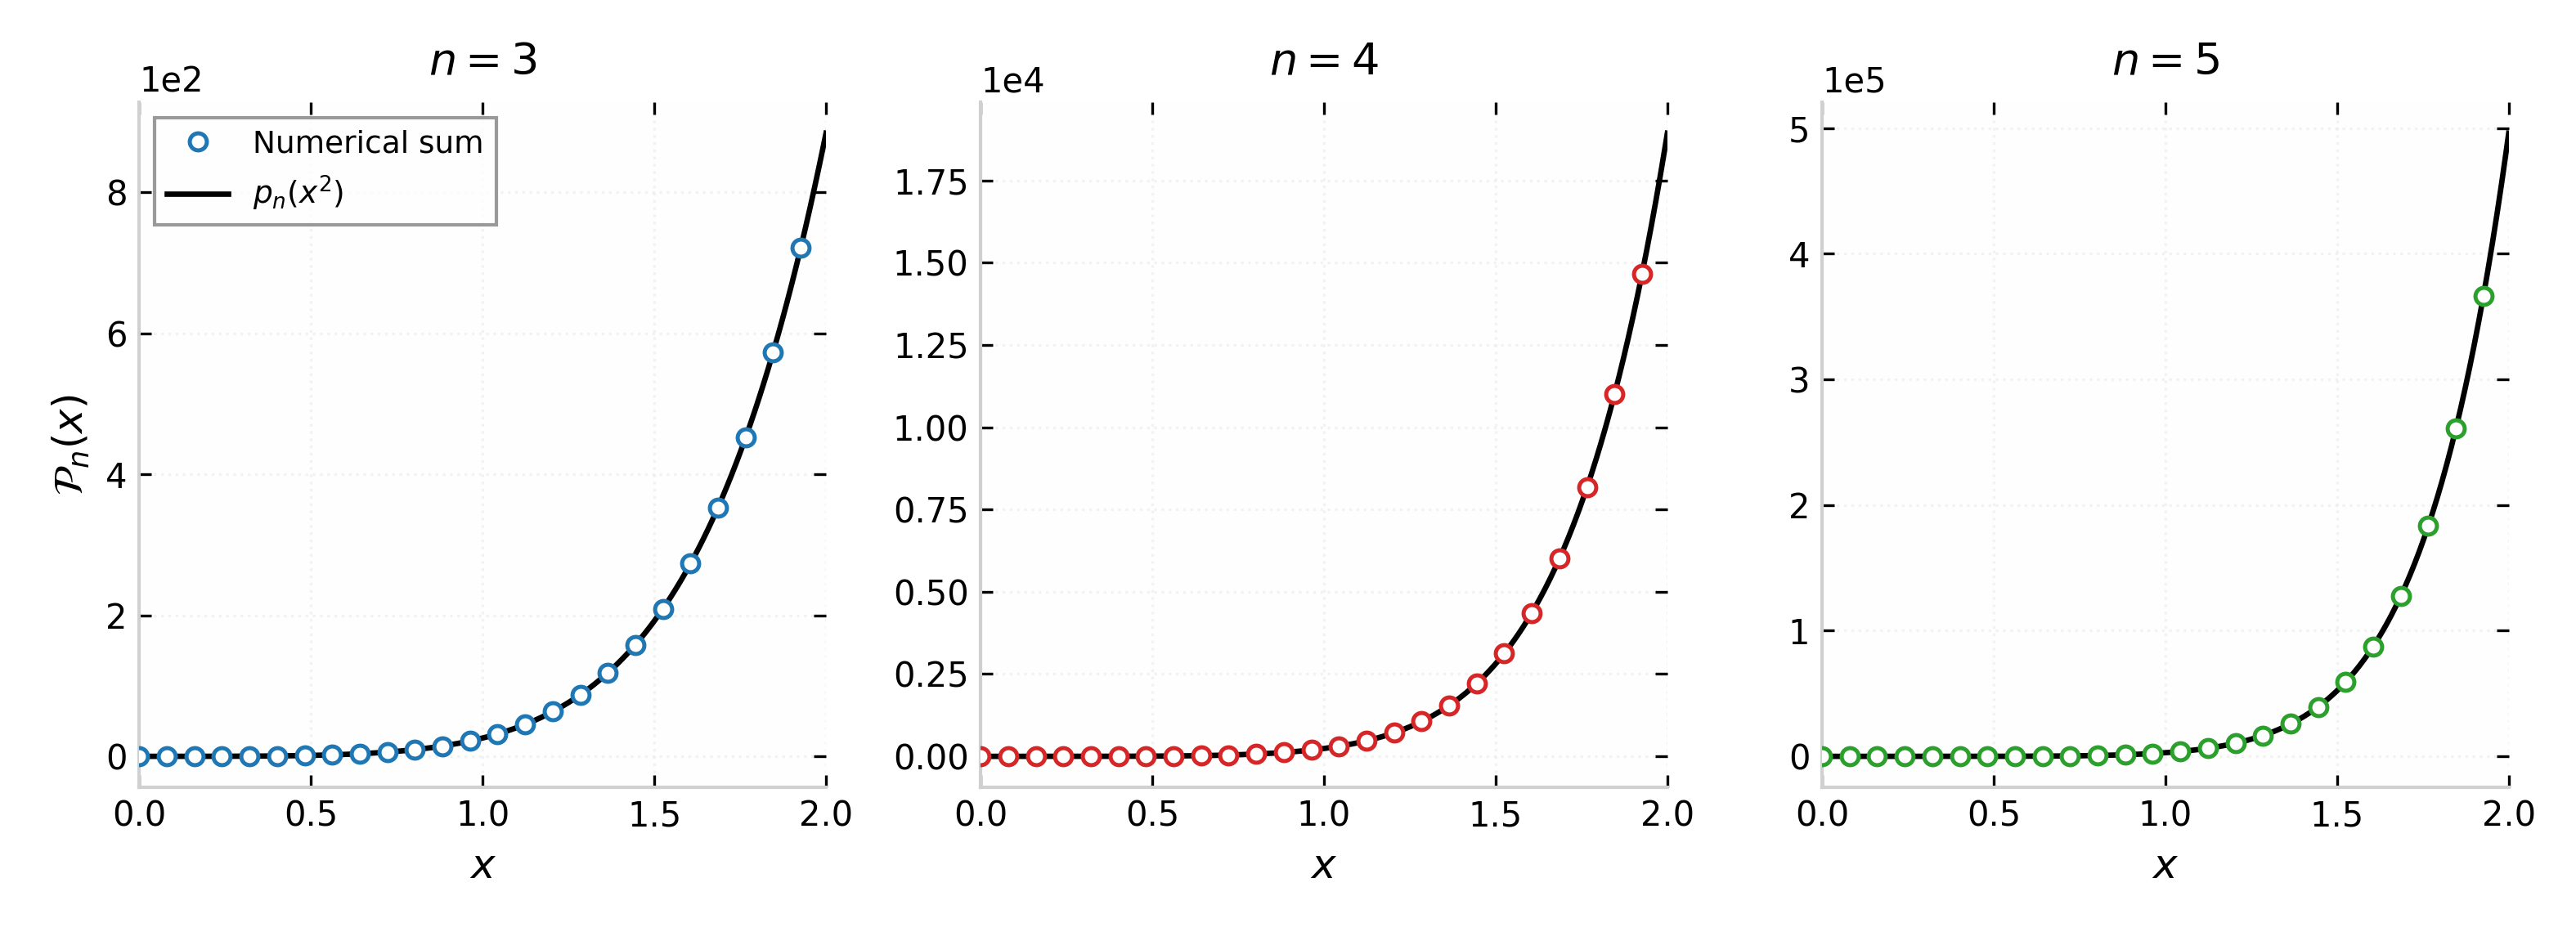
\includegraphics[width=\linewidth]{figure2.png}
\caption{Comparison of the numerical sum $\sum_{k=0}^{200}k^{2n}J_k^2(2x)$ (markers) and the 
polynomial $p_n(x^2)$ (solid curves) for $n=3,4,5$ and $0\le x\le 2$.}
\label{fig_1}
\end{figure}


\subsection{Recurrence Relation}
\label{sec:rec}

The explicit formula~\eqref{eq:coeffs} is well suited for symbolic computation, but it is also 
desirable to have a recurrence that generates the sequence $\{p_n(u)\}$ directly.  It is not difficult to show that the Bessel moment polynomials satisfy the three--term recurrence
\begin{equation}\label{eq:rec}
\boxed{\,p_{n+1}(u)=\Bigl(u\frac{d}{du}\Bigr)^{2}p_{n}(u)+4u\,p_{n}(u)-2\int_{0}^{u}p_{n}(t)\,dt\,}
\end{equation}
for $n\ge 1$ with $p_1(u)=u$.

\section{Conclusions}
\label{sec:conc}

The polynomials $p_n(u)=\sum_{k=0}^{\infty}k^{2n}\,J_k^2(2\sqrt{u})$ constitute a new family 
of moment polynomials generated by the Bessel function $J_0$.  They are not among the 
classical orthogonal polynomial families, but they enjoy several pleasant properties:
\begin{itemize}
\item explicit coefficients given by a finite alternating sum of binomial terms;
\item a compact three--term recurrence;
\item a direct combinatorial interpretation through the generating function 
$J_0(4\sqrt{u}\sin y/2)$.
\end{itemize}
Because the underlying moments arise naturally in the study of nonlinear coherent states with 
Bessel coefficients, we expect that the formulas obtained here will prove useful in future 
investigations of nonclassical light statistics and in the design of waveguide--array analogues 
of quantum optical systems.


\bigskip
\textbf{H\'ector M. Moya-Cessa }obtained his PhD at Imperial College in 1993
and since then he is a researcher/lecturer  at Instituto Nacional
de Astrof\'{\i}sica, \'Optica y Electr\'onica in Puebla, Mexico
where he works on Quantum Optics. He has published over 220 papers
in international peer reviewed journals. He is fellow of the
Alexander von Humboldt Foundation.
\begin{thebibliography}{99}

%---------------------------------------------------------------------
% Journal articles in strict MDPI format:
% Author, A.A.; Author, B.B. Title. \textit{Journal} \textbf{Year}, \textit{Volume}, pages. doi
%---------------------------------------------------------------------
\bibitem{Watson}
Watson, G.N. \textit{A Treatise on the Theory of Bessel Functions}, 2nd~ed.; 
Cambridge University Press: Cambridge, UK, 1944.

\bibitem{Gradshteyn}
Gradshteyn, I.S.; Ryzhik, I.M. \textit{Table of Integrals, Series, and Products}, 8th~ed.; 
Academic Press: Amsterdam, The Netherlands, 2014.

\bibitem{NIST}
Olver, F.W.J.; Olde Daalhuis, A.B.; Lozier, D.W.; Schneider, B.I.; Boisvert, R.F.; Clark, C.W.; Miller, B.R.; Saunders, B.V. (Eds.) 
NIST Digital Library of Mathematical Functions. 
Available online: \url{https://dlmf.nist.gov/} (accessed on 15 September 2023).

\bibitem{Axioms}
Soto-Eguibar, F.; Moya-Cessa, H.M. The Schr\"{o}dinger equation for a free particle: Generalized Bessel solutions. 
\textit{Axioms} \textbf{2025}, \textit{14}, 862.
https://doi.org/10.3390/axioms14120862

\bibitem{Jones}
Jones, A.L. Coupling of optical fibers and scattering in fibers. 
\textit{J. Opt. Soc. Am.} \textbf{1965}, \textit{55}, 261--269.
https://doi.org/10.1364/JOSA.55.000261

\bibitem{Makris}
Makris, K.G.; Christodoulides, D.N. Method of images in optical discrete systems. 
\textit{Phys. Rev. E} \textbf{2006}, \textit{73}, 036616.
https://doi.org/10.1103/PhysRevE.73.036616


\bibitem{LonghiI}
Longhi, S. Optical realization of the two-site Bose--Hubbard model in waveguide lattices. 
\textit{J. Phys. B: At. Mol. Opt. Phys.} \textbf{2011}, \textit{44}, 051001.
https://doi.org/10.1088/0953-4075/44/5/051001

\bibitem{LonghiII}
Longhi, S.; Della Valle, G.; Foglietti, V. Classical realization of two-site Fermi--Hubbard systems. 
\textit{Phys. Rev. B} \textbf{2011}, \textit{84}, 033102.
https://doi.org/10.1103/PhysRevB.84.033102

\bibitem{CrispI}
Crisp, M.D. Interaction of a charged harmonic oscillator with a single quantized electromagnetic field mode. 
\textit{Phys. Rev. A} \textbf{1991}, \textit{44}, 563--573.
https://doi.org/10.1103/PhysRevA.44.563

\bibitem{CrispII}
Crisp, M.D. Jaynes' steak dinner problem II. In \textit{Quantum Optics and Spectroscopy}; 
Cambridge University Press: Cambridge, UK, 1993; pp. 81--90.
https://doi.org/10.1017/CBO9780511524448

\bibitem{ScriptaT}
P\'{e}rez-Leija, A.; Moya-Cessa, H.M.; Christodoulides, D.N. Optical realization of the atom-field interaction in waveguide lattices. 
\textit{Phys. Scr.} \textbf{2012}, \textit{T147}, 014023.
https://doi.org/10.1088/0031-8949/2012/T147/014023
\bibitem{Several} R Juárez-Amaro, A Zúniga-Segundo, HM Moya-Cessa, Several ways to solve the Jaynes-Cummings model. App. Math. Inf. Sc. 9 , 299-303 (2015.) http://dx.doi.org/10.12785/amis/090136
\bibitem{Book} H. M. Moya-Cessa and F. Soto-Eguibar, Introduction to Quantum Optics (Rinton Press (New Jersey, 2011) ISBN 978-1-58949-061-1.

\bibitem{Jaynes}
Jaynes, E.T.; Cummings, F.W. Comparison of quantum and semiclassical radiation theories with application to the beam maser. 
\textit{Proc. IEEE} \textbf{1963}, \textit{51}, 89--109.
https://doi.org/10.1109/PROC.1963.1664

\bibitem{Shore}
Shore, B.W.; Knight, P.L. The Jaynes--Cummings model. 
\textit{J. Mod. Opt.} \textbf{1993}, \textit{40}, 1195--1238.
https://doi.org/10.1080/09500349314551321

\bibitem{Larson}
Larson, J.; Mavrogordatos, T.K. \textit{The Jaynes--Cummings Model and Its Descendants}; 
IOP Publishing: Bristol, UK, 2022.

\bibitem{Chen}
Chen, Q.-H.; Liu, T.; Zhang, Y.-Y.; Wang, K.-L. Exact solutions to the Jaynes--Cummings model without the rotating-wave approximation. 
\textit{EPL} \textbf{2011}, \textit{96}, 14003.
https://doi.org/10.1209/0295-5075/96/14003

\bibitem{BraakI}
Braak, D. Integrability of the Rabi model. 
\textit{Phys. Rev. Lett.} \textbf{2011}, \textit{107}, 100401.
https://doi.org/10.1103/PhysRevLett.107.100401

\bibitem{Anisotropic}
Ye, T.; Wang, C.; Chen, Q.-H. Anisotropic qubit-photon interactions inducing multiple antibunching-to-bunching transitions of photons. 
\textit{Opt. Express} \textbf{2024}, \textit{32}, 33483--33493.
https://doi.org/10.1364/OE.533310

\bibitem{Bocanegra}
Ivan Alejandro Bocanegra-Garay, L. Hernández-Sánchez, Irán Ramos-Prieto, Francisco Soto-Eguibar, Héctor M. Moya-Cessa, Invariant approach to the driven Jaynes--Cummings model. 
\textit{SciPost Phys.} \textbf{2024}, \textit{16}, 007.
https://doi.org/10.21468/SciPostPhys.16.1.007

\bibitem{Vidiella}
Antonio Vidiella-Barranco, Antonio Sérgio Magalhães de Castro, Alessandro Sergi, José Antonio Roversi, Antonino Messina, Agostino Migliore, Analytical solutions of the driven time-dependent Jaynes--Cummings model. 
\textit{Ann. Phys.} \textbf{2025}, \textit{537}, e00148.
https://doi.org/10.1002/andp.202500148

\bibitem{Dicke}
Dicke, R.H. Coherence in spontaneous radiation processes. 
\textit{Phys. Rev.} \textbf{1954}, \textit{93}, 99--110.
https://doi.org/10.1103/PhysRev.93.99

\bibitem{BraakII}
Braak, D. Solution of the Dicke model for $N=3$. 
\textit{J. Phys. B: At. Mol. Opt. Phys.} \textbf{2013}, \textit{46}, 224007.
https://doi.org/10.1088/0953-4075/46/22/224007


\bibitem{Lara}
Rodr\'{i}guez-Lara, B.M.; Moya-Cessa, H.M.; Klimov, A.B. Combining Jaynes--Cummings and anti-Jaynes--Cummings dynamics in a trapped-ion system driven by a laser. 
\textit{Phys. Rev. A} \textbf{2005}, \textit{71}, 023811.
https://doi.org/10.1103/PhysRevA.71.023811

\bibitem{Mayero}
Mayero, C.; Omolo, J.A. Quasi-probability distribution in light-matter interaction: The anti-Jaynes--Cummings process. 
\textit{Ann. Phys.} \textbf{2026}, \textit{488}, 170397.
https://doi.org/10.1016/j.aop.2026.170397

\bibitem{Messina}
Messina, A.; Nakazato, H.; de Castro, A.S.M.; Rocha, J.A.M.A.; Klimov, A.B.; Grimaudo, R.; Migliore, A. A generalized unitary transformation for solving time-independent and time-dependent Jaynes--Cummings models under resonant and selected off-resonance conditions. 
\textit{Ann. Phys.} \textbf{2026}, \textit{494}, 170605.
https://doi.org/10.1016/j.aop.2026.170605

\bibitem{Tsuitsui}
Tsutsui, T.T.; Cius, D.; Vidiella-Barranco, A.; de Castro, A.S.M.; Andrade, F.M. Revisiting the Jaynes--Cummings model with time-dependent coupling. 
\textit{Braz. J. Phys.} \textbf{2026}, \textit{56}, 21.
https://doi.org/10.1007/s13538-025-01487-5


\bibitem{London}
London, F. \"{U}ber die Jacobischen transformationen der quantenmechanik. 
\textit{Z. Phys.} \textbf{1926}, \textit{37}, 915--925.
https://doi.org/10.1007/BF01397491

\bibitem{Susskind}
Susskind, L.; Glogower, J. Quantum mechanical phase and time operator. 
\textit{Phys. Phys. Fiz.} \textbf{1964}, \textit{1}, 49--61.
https://doi.org/10.1007/BF00675607

\bibitem{Dattolia}
Dattoli, G.; Giannessi, L.; Richetta, M.; Torre, A. Miscellaneous results on infinite series of Bessel functions. 
\textit{Nuovo Cimento B} \textbf{1989}, \textit{103}, 149--159.
https://doi.org/10.1007/BF02891769

\bibitem{Dattolib}
Dattoli, G.; Giannessi, L.; Mezi, L.; Torre, A. Theory of generalized Bessel functions. 
\textit{Nuovo Cimento B} \textbf{1990}, \textit{105}, 327--348.
https://doi.org/10.1007/BF02723124

\bibitem{Dattolic}
Dattoli, G.; Torre, A.; Lorenzutta, S.; Maino, G.; Chiccoli, C. Theory of generalized Bessel functions---II. 
\textit{Nuovo Cimento B} \textbf{1991}, \textit{106}, 21--51.
https://doi.org/10.1007/BF02723125

\bibitem{Tapia}
Tapia-Valerdi, M.A.; Ramos-Prieto, I.; Soto-Eguibar, F.; Moya-Cessa, H.M. Waveguide arrays: Interaction to many neighbors. 
\textit{Dynamics} \textbf{2025}, \textit{5}, 25.
https://doi.org/10.3390/dynamics5030025


\bibitem{Manko}
Man'ko, M.A.; Man'ko, V.I.; Vilela Mendes, R. Nonlinear coherent states. 
\textit{Phys. Lett. A} \textbf{2001}, \textit{288}, 132--138.
https://doi.org/10.1016/S0375-9601(01)00541-6

\bibitem{RevMexFis}
Le\'{o}n-Montiel, R. de J.; Moya-Cessa, H.M.; Soto-Eguibar, F. Nonlinear coherent states for the Susskind--Glogower operators. 
\textit{Rev. Mex. F\'{i}s. S} \textbf{2011}, \textit{57}, 133--147.

\bibitem{Gazeau}
Gazeau, J.-P.; Hussin, V.; Moran, J.; Zelaya, K. Generalized Susskind--Glogower coherent states. 
\textit{J. Math. Phys.} \textbf{2021}, \textit{62}, 072104.
https://doi.org/10.1063/5.0043743

\bibitem{Mandel}
Mandel, L. Sub-Poissonian photon statistics in resonance fluorescence. 
\textit{Opt. Lett.} \textbf{1979}, \textit{4}, 205--207.
https://doi.org/10.1364/OL.4.000205


\bibitem{Fenyes}
F\'{e}nyes, I. On the moments of Bessel functions. 
\textit{Acta Math. Acad. Sci. Hung.} \textbf{1952}, \textit{3}, 285--290.
https://doi.org/10.1007/BF02022550

\bibitem{Kapteyn}
Kapteyn, W. Recherches sur les fonctions de Fourier--Bessel. 
\textit{Ann. Sci. \'{E}c. Norm. Sup\'{e}r.} \textbf{1893}, \textit{10}, 91--120.
https://doi.org/10.24033/asens.385

\bibitem{Lommel}
Lommel, E. Zur Theorie der Bessel'schen Functionen. 
\textit{Math. Ann.} \textbf{1871}, \textit{3}, 475--487.
https://doi.org/10.1007/BF01443302

\bibitem{OEIS}
Sloane, N.J.A.; et al. The On-Line Encyclopedia of Integer Sequences. 
Available online: \url{https://oeis.org} (accessed on 1 January 2024).


\end{thebibliography}

\end{document}
